\documentclass[
  bibliography=totoc,     % Literatur im Inhaltsverzeichnis
  captions=tableheading,  % Tabellenüberschriften
  titlepage=firstiscover, % Titelseite ist Deckblatt
]{scrartcl}

% Paket float verbessern
\usepackage{scrhack}

% Warnung, falls nochmal kompiliert werden muss
\usepackage[aux]{rerunfilecheck}

% unverzichtbare Mathe-Befehle
\usepackage{amsmath}
% viele Mathe-Symbole
\usepackage{amssymb}
% Erweiterungen für amsmath
\usepackage{mathtools}

% Fonteinstellungen
\usepackage{fontspec}
% Latin Modern Fonts werden automatisch geladen
% Alternativ:
%\setromanfont{Libertinus Serif}
%\setsansfont{Libertinus Sans}
%\setmonofont{Libertinus Mono}
\recalctypearea % Wenn man andere Schriftarten gesetzt hat,
% sollte man das Seiten-Layout neu berechnen lassen

% deutsche Spracheinstellungen
\usepackage{polyglossia}
\setmainlanguage{german}


\usepackage[
  math-style=ISO,    % ┐
  bold-style=ISO,    % │
  sans-style=italic, % │ ISO-Standard folgen
  nabla=upright,     % │
  partial=upright,   % ┘
  warnings-off={           % ┐
    mathtools-colon,       % │ unnötige Warnungen ausschalten
    mathtools-overbracket, % │
},                       % ┘
]{unicode-math}

% traditionelle Fonts für Mathematik
\setmathfont{Latin Modern Math}
% Alternativ:
%\setmathfont{Libertinus Math}

\setmathfont{XITS Math}[range={scr, bfscr}]
\setmathfont{XITS Math}[range={cal, bfcal}, StylisticSet=1]

% Zahlen und Einheiten
\usepackage[
locale=DE,                   % deutsche Einstellungen
separate-uncertainty=true,   % immer Fehler mit \pm
per-mode=symbol-or-fraction, % / in inline math, fraction in display math
]{siunitx}

% chemische Formeln
\usepackage[
version=4,
math-greek=default, % ┐ mit unicode-math zusammenarbeiten
text-greek=default, % ┘
]{mhchem}

% richtige Anführungszeichen
\usepackage[autostyle]{csquotes}

% schöne Brüche im Text
\usepackage{xfrac}

% Standardplatzierung für Floats einstellen
\usepackage{float}
\floatplacement{figure}{htbp}
\floatplacement{table}{htbp}

% Floats innerhalb einer Section halten
\usepackage[
section, % Floats innerhalb der Section halten
below,   % unterhalb der Section aber auf der selben Seite ist ok
]{placeins}

% Seite drehen für breite Tabellen: landscape Umgebung
\usepackage{pdflscape}

% Captions schöner machen.
\usepackage[
  labelfont=bf,        % Tabelle x: Abbildung y: ist jetzt fett
  font=small,          % Schrift etwas kleiner als Dokument
  width=0.9\textwidth, % maximale Breite einer Caption schmaler
]{caption}
% subfigure, subtable, subref
\usepackage{subcaption}

% Grafiken können eingebunden werden
\usepackage{graphicx}
% größere Variation von Dateinamen möglich
\usepackage{grffile}

% schöne Tabellen
\usepackage{booktabs}

% Verbesserungen am Schriftbild
\usepackage{microtype}

% Literaturverzeichnis
\usepackage[style=alphabetic,]{biblatex}
% Quellendatenbank
\addbibresource{lit.bib}
\addbibresource{programme.bib}

% Hyperlinks im Dokument
\usepackage[
  unicode,        % Unicode in PDF-Attributen erlauben
  pdfusetitle,    % Titel, Autoren und Datum als PDF-Attribute
  pdfcreator={},  % ┐ PDF-Attribute säubern
  pdfproducer={}, % ┘
]{hyperref}
% erweiterte Bookmarks im PDF
\usepackage{bookmark}

% Trennung von Wörtern mit Strichen
\usepackage[shortcuts]{extdash}

\title{V602: Röntgenemission und -absorption}
\author{
  Simon Schulte
  \texorpdfstring{
    \\
    \href{mailto:simon.schulte@udo.edu}{simon.schulte@udo.edu}
  }{}
  \texorpdfstring{\and}{, }
  Tim Sedlaczek
  \texorpdfstring{
    \\
    \href{mailto:tim.sedlaczek@udo.edu}{tim.sedlaczek@udo.edu}
  }{}
}
\publishers{TU Dortmund – Fakultät Physik}

\date{Durchführung: 30.05.2017\\
      Abgabe: 06.06.2017\\
      Korrektur: 21.06.2017}


\begin{document}

\maketitle
\thispagestyle{empty}
\tableofcontents
\newpage
\setcounter{page}{1}
\section{Zielsetzung}
\label{sec:zielsetzung}
In diesem Versuch wird das Emissionsspektrum einer Kupfer-Röntgenröhre
und verschiedene Absorptionsspektren untersucht.
\section{Theorie}
\label{sec:theorie}
Röntgenstrahlung besteht aus elektromagnetischen Wellen im Energiebereich von
mehreren $\si{\kilo\electronvolt}$. Sie wird erzeugt, indem Elektronen eine
entsprechend große Beschleunigungsspannug durchlaufen und anschließend auf die
Anode treffen. Im Coulombfeld der Kerne des Anodenmaterials werden die Elektronen
abgebremst. Dabei geben diese dann einen Teil ihrer Energie in Form von
Röntgenstrahlung ab. Da die Elektronen dabei einen beliebigen Teil ihrer Energie
abgeben können ist dieses Spektrum kontinuierlich. Es wird allgemein als
Bremsspektrum bezeichnet. Die maximale Energie, der Röntgenstrahlung, entspricht
dabei der kinetischen Energie der Elektronen. Da sich die Strahlungsenergie
antiproportional zur Wellenlänge verhält, äußert sich dies in einer minimalen
Wellenlänge:
\begin{equation}
  \lambda_\mathup{min} = \frac{h \cdot c}{e_0 U}.
  \label{eqn:minlam}
\end{equation}
Dabei ist $E_\mathup{kin} = e_0 U$ die kinetische Energie der Elektronen und
$E = h \cdot \nu$, mit der Frequenz $\nu$, die Energie der Strahlung.
In Abbildung \ref{fig:V6021} ist ein solches Bremsspektrum schematisch
dargestellt.
\begin{figure}[htb]
  \centering
  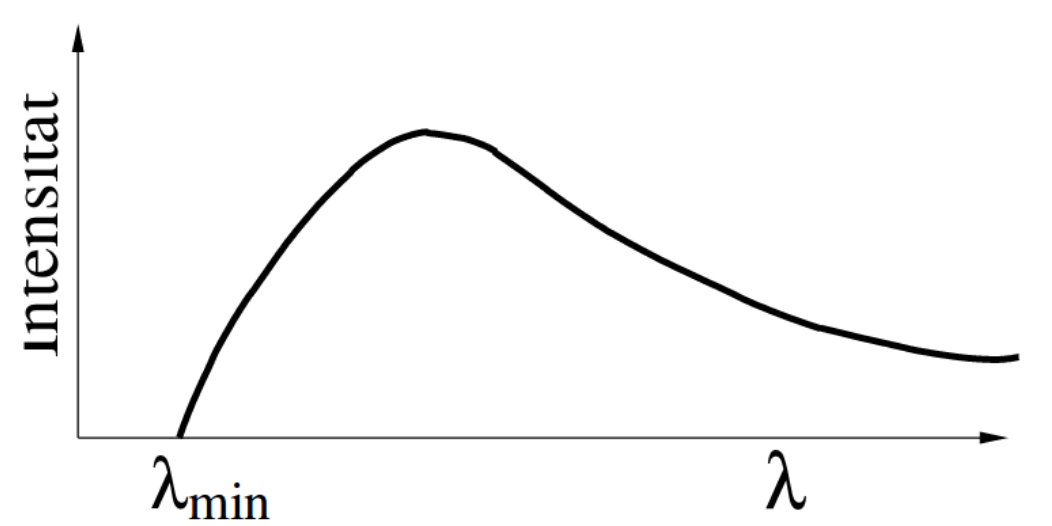
\includegraphics[width=0.6\textwidth]{V6021.png}
  \caption{Schema des Bremsspektrums. \cite{anleitung}}
  \label{fig:V6021}
\end{figure}

\noindent
Für das sogenannte charakteristische Spektrum geben die Elektronen ihre Energie
an eines der inneren Hüllenelektronen das Anodenmaterials ab. Diese werden
dadurch ionisiert und ein äußeres Elektron rückt dafür nach. Bei dem abfallen
auf das energetisch günstigere Niveau gibt es dann den Wert der
Energiedifferenz in Form von Röntgenstrahlung ab:
\begin{equation}
  h \nu = E_m - E_n.
  \label{eqn:energdif}
\end{equation}
Das charakteristische Spektrum zeichnet sich deshalb durch scharfe, diskrete
Peaks aus. Für diese Peaks werden verschiedene Bezeichnungen verwendet, die
darauf basieren, von welchem Zustand in welchen anderen Zustand der Übergang
stattfindet. Z.B. werden die Bezeichnungen $K_\alpha$, $K_\beta$, $L_\alpha$,
$L_\beta$ usw. verwendet. Der Buchstabe steht dabei jeweils für den energetisch
günstigeren Zustand, auf den das Elektron herabfällt. Sie sind von $K$ aus
aufwärts alphabetisch nummeriert. Die griechischen Indizes stehen für den
Ursprung des Elektrons. So bedeutet der $K_\alpha$-Übergang, dass ein Elektron
aus der $L$-Schale in die $K$-Schale wandert, und der $K_\beta$-Übergang, dass
ein Elektron aus der $M$-Schale in die $K$-Schale wandert.

\noindent
Die Bindungsenergie der Elektronen im Anodenmaterial wird durch innere
Elektronen
geschwächt. Daher ergibt sich für diese:
\begin{equation}
  E_n = - R_\infty z_{eff}^2 \cdot \frac{1}{n^2}.
  \label{eqn:bindungsen}
\end{equation}
Dabei ist $z_{eff} = z - \sigma$ die effektive Kernladungszahl, mit der
Abschirmkonstante $\sigma$, und $R_\infty = \SI{13.6}{\electronvolt}$ die
Rydbergenergie. Der Index $n$ nimmt von $K = 1$ aus aufsteigend ganze Zahlen
an.
Die Spektren treten parallel auf, weshalb sich das Emissionsspektrum aus beiden
zusammensetzt.

\noindent
Das Absorpionsspektrum von Röntgenstrahlung ist ebenfalls sehr
materialabhängig.
Allgemein nimmt das Absorptionsvermögen eines Absorbers mit zunehmender Energie
ab. Es steigt jedoch abrupt, wenn die Strahlung die Ionisierungsenergie einer
weiter innen gelegenen Schale erreicht. Dadurch werden sich dort befindliche
Elektronen ionisiert. Die Absorptionskanten werden nach der
Schale benannt, aus der das entsprechende Elektron stammt.
Ein Schema des Absorptionsvermögens ist in Abbildung \ref{fig:V6022}
dargestellt.
\begin{figure}[htb]
  \centering
  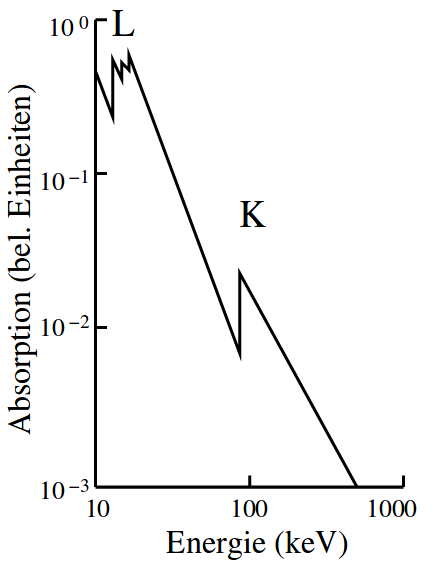
\includegraphics[width=0.45\textwidth]{V6022.png}
  \caption{K- und L-Absorptionskante. \cite{anleitung}}
  \label{fig:V6022}
\end{figure}

\noindent
Die Position der Kanten ist mit
\begin{equation}
  h \nu_{abs} = E_n - E_\infty
  \label{eqn:abskante}
\end{equation}
gegeben.

\noindent
Theoretisch setzen sich die Kanten aus mehreren leicht versetzten Linien
zusammen. Das liegt daran, dass die Bindungsenergie, aufgrund des Spins und
des Bahndrehimpulses, innerhalb einer Schale leicht variiert. Mehrere Kanten
sind jedoch praktisch nur bei den $L$-Kanten zu beobachten. Dabei ist dann die
Sommerfeld'sche Feinstrukturformel
\begin{equation}
  E_{n,j} = - R_\infty \left( z_{eff,1}^2 \cdot \frac{1}{n^2} + \alpha^2 z_{eff,2}^4 \cdot \frac{1}{n^3} \left( \frac{1}{j+\frac{1}{2}} - \frac{3}{4n} \right) \right)
  \label{eqn:sommerfeld}
\end{equation}
für die Bindungsenergien zu beachten.
Das $\alpha$ steht für die Sommerfeld'sche Feinstrukturkonstante und $j$ für
den Gesamtdrehimpuls des Elektrons.
Für die zweite effektive Kernladungszahl $z_{eff,2}$ wird eine neue
Abschirmkonstante $\sigma_L$ benötigt.
Diese berechnet sich nach:
\begin{equation}
  \sigma_L = Z - \left( \frac{4}{\alpha} \sqrt{\frac{\Delta E_L}{R_\infty}} -
  \frac{5 \Delta E_L}{R_\infty} \right)^\frac{1}{2} \left( 1+ \frac{19}{32}
  \alpha^2 \frac{\Delta E_L}{R_\infty} \right)^\frac{1}{2}.
  \label{eqn:sigl}
\end{equation}
Hierbei ist $\Delta E_L = E_{L_{II}} - E_{L_{III}}$ die Energiedifferenz
zwischen
der $L_{II}$ und der $L_{III}$ Kante und $Z$ die Ordnungszahl des Absorbers.

\noindent
Bei diesem Versuch wird für die Messung der Spektren ein Effekt ausgenutzt, der
Bragg'sche Reflexion genannt wird. Hierbei wird die Röntgenstrahlung an den
verschiedenen Gitterebenen eines LiF-Kristalls reflektiert. Durch den dabei
entstehenden Gangunterschied interferieren die Röntgenwellen. Nach
\begin{equation}
  2 d \sin \theta = n \lambda
  \label{eqn:bragg}
\end{equation}
lässt sich dann aus dem Glanzwinkel $\theta$ und der Gitterkonstante $d$ die
Wellenlänge der Röntgenstrahlung bestimmen. In Abbildung \ref{fig:V6023} ist
dies schematisch dargestellt.
\begin{figure}[htb]
  \centering
  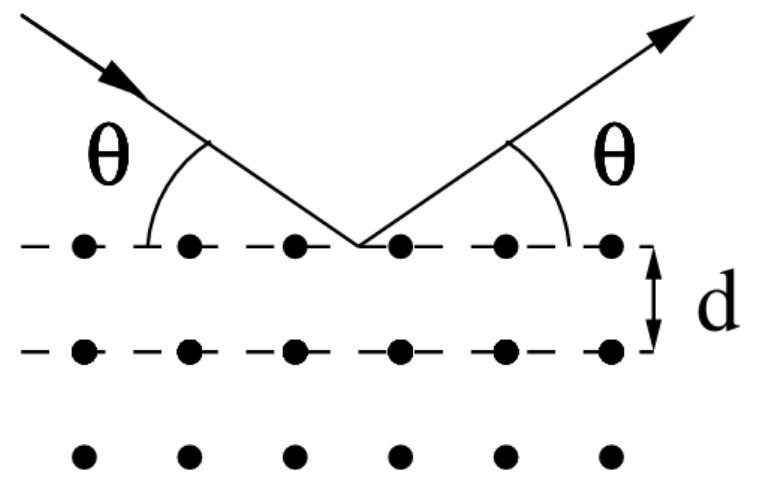
\includegraphics[width=0.5\textwidth]{V6023.png}
  \caption{Schema der Bragg'schen Reflexion. \cite{anleitung}}
  \label{fig:V6023}
\end{figure}
\clearpage
\section{Durchführung}
\label{sec:durchführung}
\subsection{Versuchsaufbau}
\label{sec:aufbau}
In Abbildung \ref{fig:V6024} ist der Aufbau der Apparatur dargestellt.
\begin{figure}[htb]
  \centering
  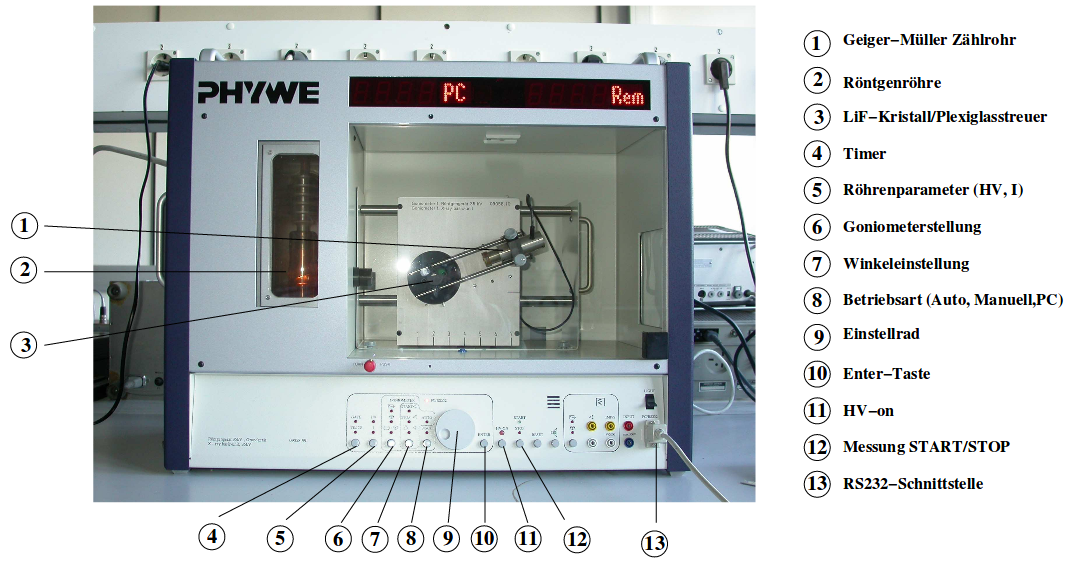
\includegraphics[width=\textwidth]{V6024.png}
  \caption{Aufbau der Apparatur. \cite{anleitung}}
  \label{fig:V6024}
\end{figure}
Die Röntgenröhre (2) erzeugt Röntgenstrahlung. Diese wird am Kristall (3)
reflektiert und am Geiger-Müller-Zählrohr (1) wird die Intensität gemessen.
Für die Messung der Absorptionsspektren lässt sich am Geiger-Müller-Zählrohr
ein entsprechender Absorber befestigen. Die Schalter an der unteren Seite der
Apparatur (4-13) werden für den Versuch nicht benötigt, da die Apparatur mit
einem Computer gesteuert wird.
\subsection{Versuchsablauf}
\label{sec:ablauf}
Zu Beginn wird die Bragg'sche Bedingung überprüft, indem der Kristall auf einen
Winkel von $\SI{14}{\degree}$ fest eingestellt wird und dann die Intensität
für Zählrohrwinkel $\alpha_{GM}$ von $\SI{26}{\degree}$ bis $\SI{30}{\degree}$
in $\SI{0.2}{\degree}$-Schritten gemessen wird. Im Idealfall sollte das Maximum
der Intensität bei $\SI{28}{\degree}$ liegen.\\

\noindent
Für alle weiteren Messungen wird der 2:1 Koppelmodus verwendet.
Das bedeutet, dass der Zählrohrwinkel immer den doppelten Winkel des Kristalls
annimmt. Dadurch wird die Intensität immer am Interferenzmaximum gemessen.
Nun wird das Emissionsspektrum der Röntgenröhre gemessen.
Hierzu wird die Intensität bei einem Kristallwinkel von $\SI{4}{\degree}$ bis
$\SI{26}{\degree}$ in $\SI{0.2}{\degree}$-Schritten gemessen. Als Integrationszeit
pro Winkel wird $\Delta t = \SI{5}{\second}$ verwendet.\\

\noindent
Für die Messung der Absorptionsspektren wird jeweils ein Absorber am
Zählrohr befestigt. Vor der Messung wird nach Literaturwerten jeweils der
theoretische Winkel der Absorptionskante, die beobachtet werden soll, bestimmt.
Dieser Wert wird auf eine ganze Zahl gerundet und die Intensität im Bereich
von $\pm \SI{2}{\degree}$ um den Wert herum in $\SI{0.1}{\degree}$-Schritten
gemessen. Dabei wird eine Integrationszeit von $\Delta t = \SI{20}{\second}$
verwendet. Es werden die $K$-Kanten von 4 leichten Elementen ($30 \leq Z \leq 50$)
vermessen und die $L_{II}$- und $L_{III}$-Kanten eines schweren Elements.
Bei dem schweren Element wird die Intensität im Bereich von $\pm \SI{3}{\degree}$
um die beiden Kanten gemessen. Die Schrittweite sowie die Integrationszeit
bleiben dabei gleich. Die verwendeten Elemente und Winkelbereiche stehen
in Tabelle \ref{tab:elemuwink}.
\begin{table}
  \centering
  \caption{Verwendete Elemente und Winkel.}
  \label{tab:elemuwink}
  \sisetup{table-format=2.0}
  \begin{tabular}{S S S}
    \toprule
    {Element} & {Z} & {Winkelbereich von $\theta$ in $\si{\degree}$} \\
    \midrule
    \text{Germanium (Ge)} & 32 & $\SI{14}{\degree} \; \text{bis} \; \SI{18}{\degree}$ \\
    \text{Zirconium (Zr)} & 40 & $\SI{8}{\degree} \; \text{bis} \; \SI{12}{\degree}$ \\
    \text{Zink (Zn)} & 30 & $\SI{17}{\degree} \; \text{bis} \; \SI{21}{\degree}$ \\
    \text{Brom (Br)} & 35 & $\SI{11}{\degree} \; \text{bis} \; \SI{15}{\degree}$ \\
    \text{Bismut (Bi)} & 83 & $\SI{8}{\degree} \; \text{bis} \; \SI{16}{\degree}$ \\
    \bottomrule
  \end{tabular}
\end{table}
\clearpage
\section{Auswertung}
\label{sec:auswertung}
\begin{figure}[H]
  \centering
  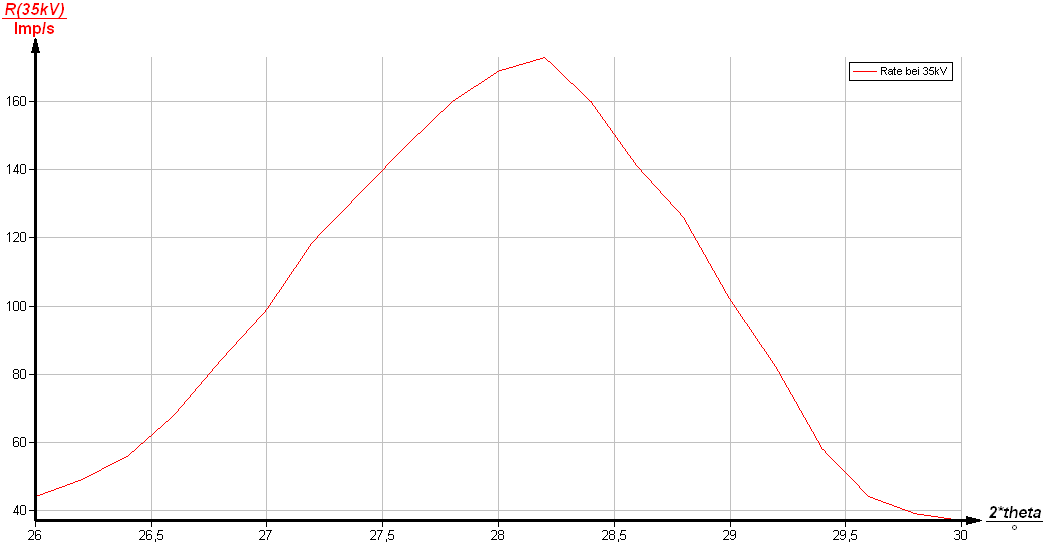
\includegraphics[width=0.9\textwidth]{1.png}
  \caption{Überprüfung der Bragg Bedingung.}
  \label{fig:6025}
\end{figure}
Das Maximum des Graphen in Abbildung \ref{fig:6025} liegt bei etwa \SI{14.1}{°}.
\begin{figure}[H]
  \centering
  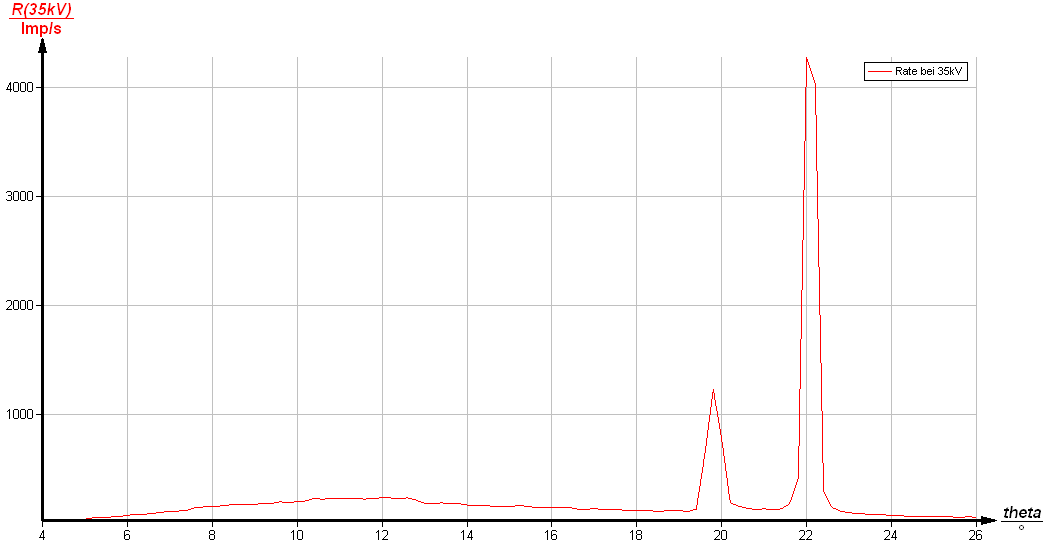
\includegraphics[width=0.9\textwidth]{Emission.png}
  \caption{Das Emissionsspektrum von Kupfer.}
  \label{fig:60211}
\end{figure}
\noindent
Abbildung \ref{fig:60211} zeigt das Emissionsspektrum einer Cu-Röntgenröhre. Es beginnt bei $5°$ und endet bei $26°$. Die $K_{\alpha}$-und $K_{\beta}$-Linien sind in den beiden Bergen enthalten. Dabei liegt $K_{\alpha}$ bei $22°$ und $K_{\beta}$ bei $19.8°$. Das Maximum von $K_{\alpha}$ entspricht einem Wert von $\SI{4273.0}{\frac{Impulse}{s}}$ und das Maximum von $K_{\beta}$ entspricht
einem Wert von $\SI{1228}{\frac{Impulse}{s}}$. Durch Gleichung \eqref{eqn:minlam} wird außerdem $E_{max}$ und der Sollwert bestimmt. Dabei ergibt sich für den Sollwert
\begin{equation*}
  e_0 U\,=\,\SI{35000}{\electronvolt}
\end{equation*}
und für $E_{max}$ ergibt sich mit Formel~\eqref{eqn:energie}
\begin{equation}
  E\,=\,\frac{hc}{2d\sin\theta}
  \label{eqn:energie}
\end{equation}
ein Wert von
\begin{equation*}
  E_{max}\,=\,\SI{32001}{\electronvolt}.
\end{equation*}
Die Abweichung beträgt dabei etwa \SI{8.6}{\percent}. Außerdem werden die Halbwertsbreiten berechnet. Dafür werden die Winkel gesucht, an denen genau die Hälfte des Maximums zu finden ist. Für die Energien wird die Formel
\begin{equation}
  E\,=\,\frac{hc}{2d\sin\theta}
\end{equation}
benutzt. Dann ergibt sich Tabelle \ref{tab:energiedifferenzen}.
\begin{table}[H]
	\begin{center}
	\caption{Die berechneten Werte für die Energiedifferenzen.}
	\label{tab:energiedifferenzen}
		\begin{tabular}{cccc}
			\toprule
			{Wert} & {Winkel $\theta$ [°]} & {Energie [$eV$]}
      & {Energiedifferenz $\delta$E [eV]}\\
			\midrule
      $K_{\beta 1}$ & $19,4$ & $9619$ & $/$ \\
			$K_{\beta 2}$ & $20,2$ & $9253$ & $366$ \\
			$K_{\alpha 1}$ & $21,6$ & $8679$ & $/$\\
			$K_{\alpha 2}$ & $22,4$ & $8385$ & $294$ \\
			\bottomrule
		\end{tabular}
	\end{center}
\end{table}
\noindent
Dabei bezeichnet $K_{\beta 1}$ den Anfang des $\beta$-Bergs und $K_{\beta 2}$ das Ende des $\beta$-Bergs. Das gleiche gilt für $K_{\alpha 1}$ und $K_{\alpha 2}$. Die Energiedifferenzen aus Tabelle \ref{tab:energiedifferenzen} sind auch die Halbwertsbreiten für $K_{\alpha}$- und $K_{\beta}$- Linien. Dabei beträgt die Energie an den Maxima:
\begin{align*}
  E_{K_{\beta}}\,=\,\SI{9432}{\electronvolt} \\
  E_{K_{\alpha}}\,=\,\SI{8529}{\electronvolt}.
\end{align*}
Es wird außerdem nach der Aussage des Auflösungsvermögens gefragt. Das Auflösungsvermögen ist der grundsätzliche Abstand zweier Strukturen, ab dem erkennbar ist, dass es sich um zwei von diesen handelt. Außerdem sollen die Abschirmkonstanten $\sigma$ bestimmt werden. Dafür werden die Formeln
\begin{equation}
  \sigma_1\,=\,z_{Cu}-\sqrt{\frac{E_{K_{\beta}}}{R_{\infty}}}
\end{equation}
und
\begin{equation}
  \sigma_2\,=\,z_{Cu}-\sqrt{- \frac{4(E_{K_{\alpha}}-E_{K_{\beta}})}{R_{\infty}}}
\end{equation}
genutzt.
\noindent
Dann ergibt sich für die beiden Werte:
\begin{align*}
  \sigma_{1}\,=\,2.66 \\
  \sigma_{2}\,=\,12.70.
\end{align*}
Im Folgenden sind die Graphen für die Absorptionsspektren von Brom, Germanium, Zink und Zirkonium zu sehen.
\begin{figure}[H]
  \centering
  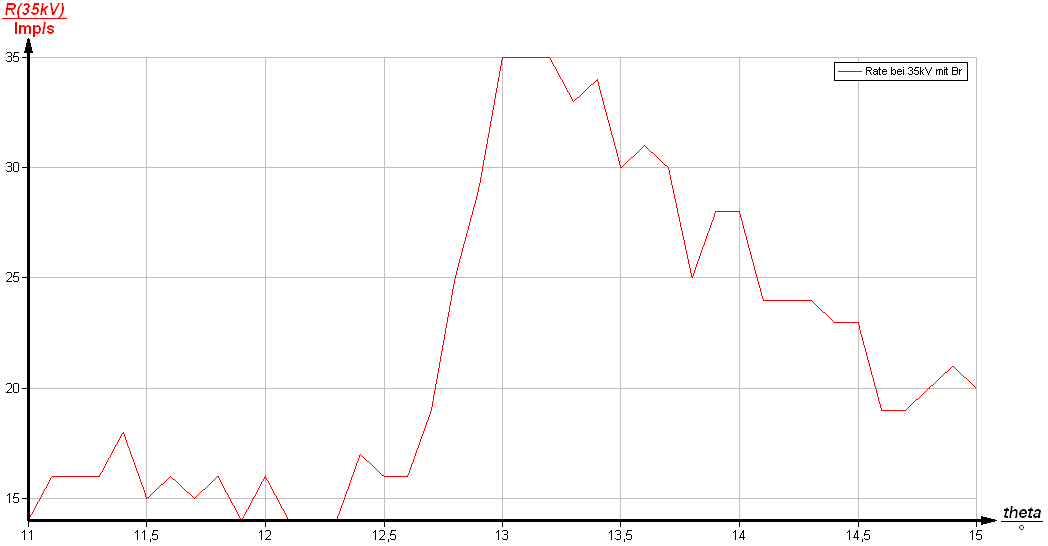
\includegraphics[width=0.9\textwidth]{AbsBr.png}
  \caption{Das Absorptionsspektrum von Brom.}
  \label{fig:6027}
\end{figure}
\begin{figure}[H]
  \centering
  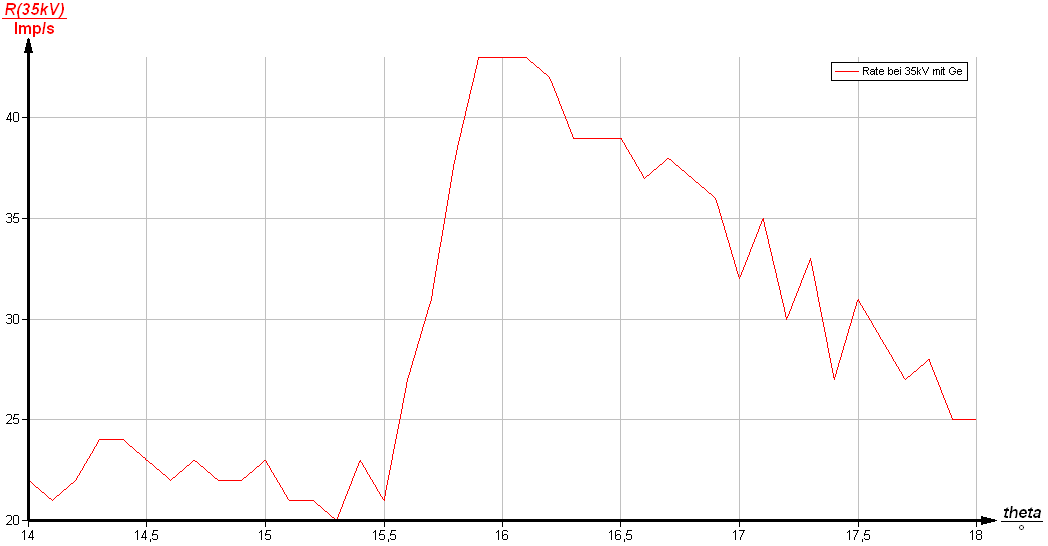
\includegraphics[width=0.9\textwidth]{AbsGe.png}
  \caption{Das Absorptionsspektrum von Germanium.}
  \label{fig:6028}
\end{figure}
\begin{figure}[H]
  \centering
  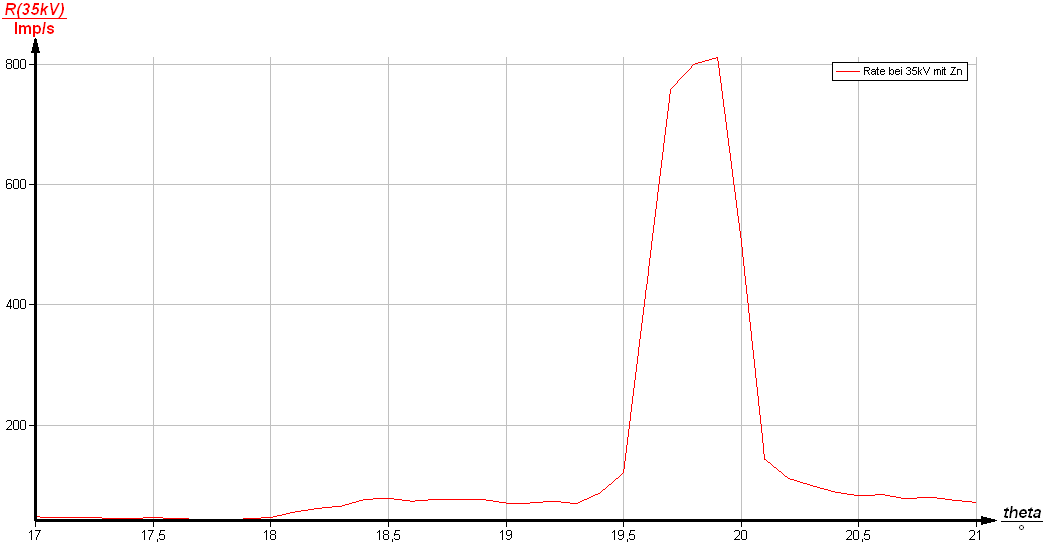
\includegraphics[width=0.9\textwidth]{AbsZn.png}
  \caption{Das Absorptionsspektrum von Zink.}
  \label{fig:6029}
\end{figure}
\begin{figure}[H]
  \centering
  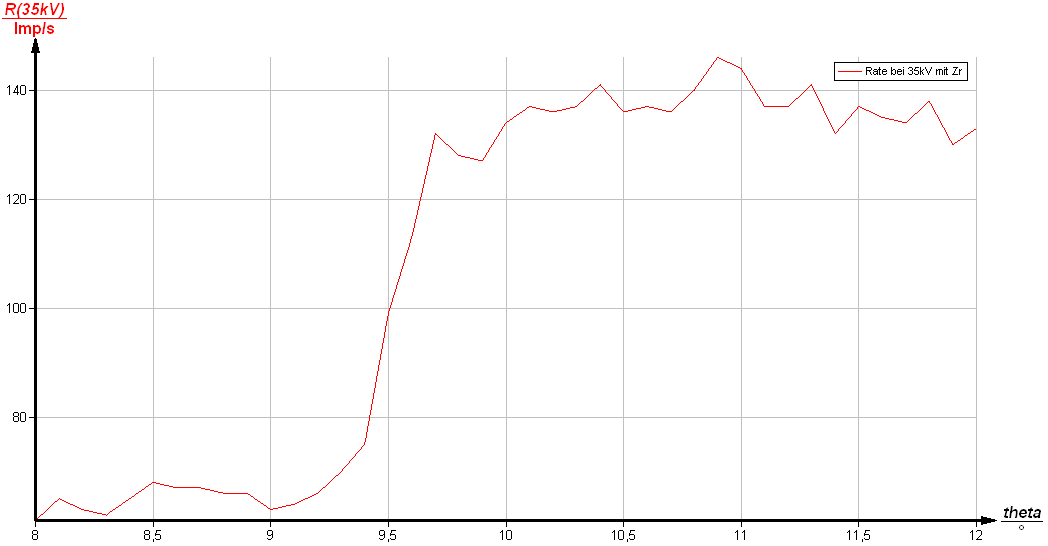
\includegraphics[width=0.9\textwidth]{AbsZr.png}
  \caption{Das Absorptionsspektrum von Zirkonium.}
  \label{fig:60210}
\end{figure}
\noindent
Das sind sogenannte leichte Absorber. Auch hier wird wieder $\sigma$ bestimmt. Dafür wird die Formel
\begin{equation}
  \sigma\,=\,z-\sqrt{\frac{E_k}{R_{\infty}}- \frac{\alpha^4 z^4}{4}}
\end{equation}
genutzt.
\noindent
Das $\alpha$ in dieser Formel ist dabei stets $\alpha$\,=\,$\frac{1}{137}$. Das ist die Sommerfeld'sche Feinstrukturkonstante. Tabelle \ref{tab:errechnet} zeigt die errechneten Werte.
\begin{table}[H]
	\begin{center}
	\caption{Die berechneten Werte für die Abschirmkonstanten und Energien der leichten Absorber.}
	\label{tab:errechnet}
		\begin{tabular}{ccccc}
			\toprule
      {Ordnungszahl} & {Element} & {Winkel $\theta$ [°]} & {Energie [$eV$]}
      & {Abschirmkonstante $\sigma$}\\
			\midrule
      30  & Zink & $18,1$ & $10017$ & $3,06$ \\
      32  & Germanium & $16,0$ & $11522$ & $3,13$\\
      35  & Brom & $13,2$ & $13992$ & $3,24$ \\
      40  & Zirkonium & $10,9$ & $18584$ & $3,50$ \\
			\bottomrule
		\end{tabular}
	\end{center}
\end{table}
\noindent
Der Zusammenhang zwischen der Energie und der Ordnungszahl wird dabei auch in Abbildung \ref{plot} dargestellt
\begin{figure}[H]
  \centering
  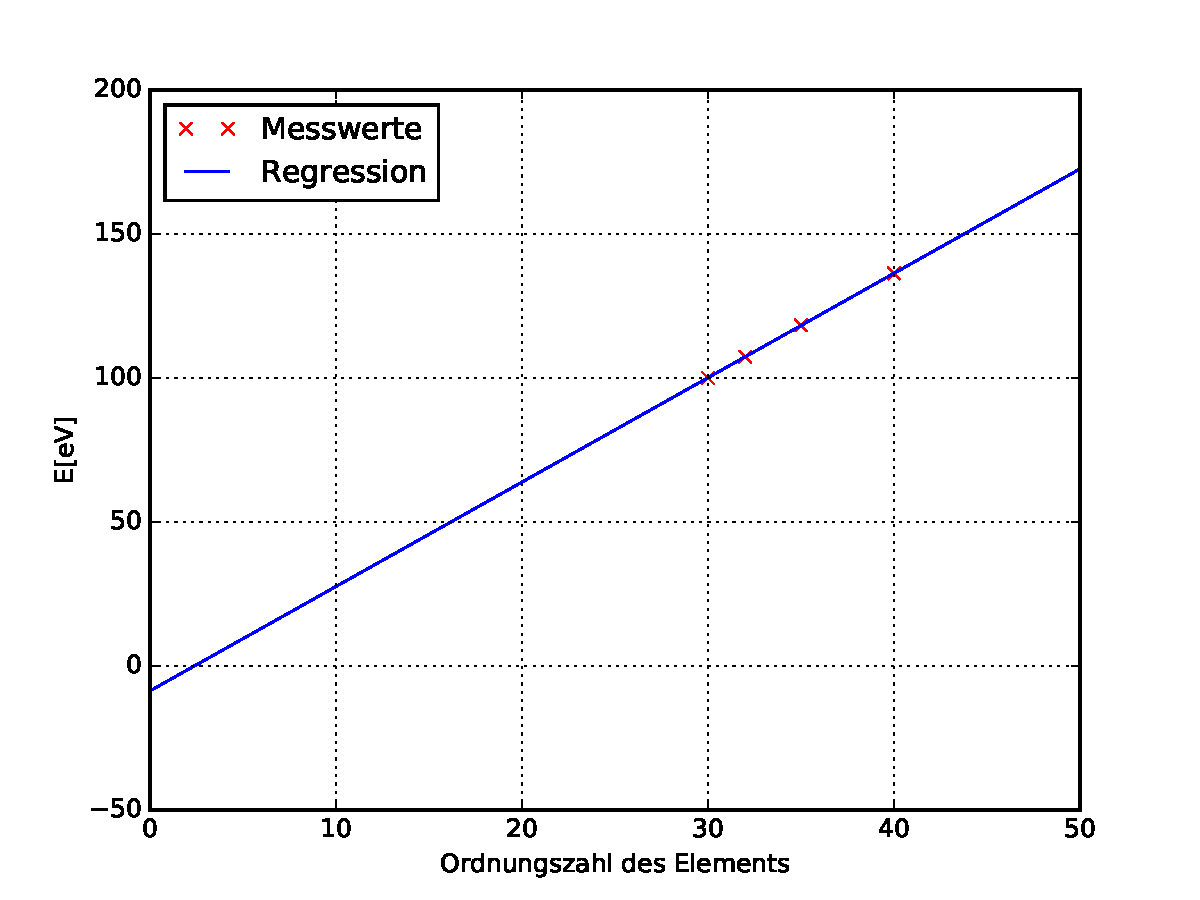
\includegraphics[width=0.9\textwidth]{plot.pdf}
  \caption{Der Zusammenhang zwischen der Ordnungszahl und der Energie eines Elements.}
  \label{plot}
\end{figure}
Dabei ergibt sich:
\begin{align*}
  a\,=\,\SI{3.63(1)}{\sqrt{eV}} \\
  b\,=\,\SI{-8.64(24)}{\sqrt{eV}}
\end{align*}
Dabei soll $a$ quadriert gleich der Rydberg-Energie $R_{\infty}$ sein.
\begin{equation*}
  a²\,=\,\SI{13.10(4)}{eV}
\end{equation*}
Als nächstes werden schwere Absorber betrachtet.
\begin{figure}[H]
  \centering
  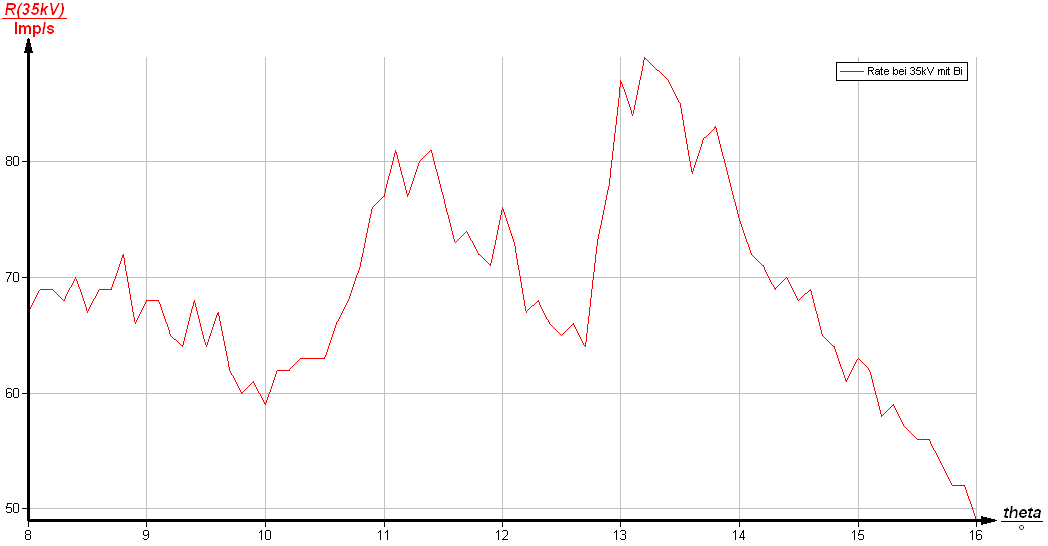
\includegraphics[width=0.9\textwidth]{AbsBi.png}
  \caption{Das Absorptionsspektrum von Bismut.}
  \label{fig:6026}
\end{figure}
\noindent
Abbildung \ref{fig:6026} zeigt das Absorptionsspektrum von Bismut. Dabei liegen die L-Kanten bei den Winkeln
\begin{align*}
  \theta_{L1}\,=\,11.1° \\
  \theta_{L2}\,=\,13.2°
\end{align*}
Die dazu berechneten Energien und die dazu gehörige Energiedifferenz lauten
\begin{align*}
  E_{L1}\,=\,\SI{16596}{\electronvolt} \\
  E_{L2}\,=\,\SI{13992}{\electronvolt} \\
  \symup{\Delta} E_L\,=\,\SI{2604}{\electronvolt}.
\end{align*}
Mit Formel~\eqref{eqn:sigl} wird nun noch die Abschirmkonstante von Bismut berechnet. Für diese ergibt sich
\begin{equation*}
  \sigma_L\,=\,4,15.
\end{equation*}
Dabei ist der Literaturwert
\begin{equation*}
  \sigma_{\symup{Lit}}\,=\,4,19.
\end{equation*}
\newpage
\section{Diskussion}
\label{sec:diskussion}
Als erstes wurde die Bragg-Bedingung überprüft. Dabei sollte das Maximum eigentlich bei einem Winkel von etwa $28°$ liegen. Gemessen wurde ein Wert von $28.2°$. Das ist eine Abweichung von unter \SI{1}{\percent}. Es ist davon auszugehen, dass somit die Bedingung bestätigt wurde.
Als nächstes werden die leichten Absorber betrachtet. Tabelle \ref{tab:literaturwerte} zeigt die Literaturwerte \cite{wissen} für die Abschirmkonstanten.
\begin{table}[H]
	\begin{center}
	\caption{Die Literaturwerte für die Abschirmkonstanten und Energien leichter Absorber.}
	\label{tab:literaturwerte}
		\begin{tabular}{ccccc}
			\toprule
			{Ordnungszahl} & {Element} & {Winkel $\theta$ [°]} & {Energie [$eV$]}
      & {Abschirmkonstante $\sigma$}\\
			\midrule
			30  & Zink & $18,6$ & $9650$ & $3,56$ \\
			32  & Germanium & $16,1$ & $11100$ & $3,56$\\
			35  & Brom & $13,2$ & $18980$ & $3,85$ \\
			40  & Zirkonium & $9,9$ & $17990$ & $4,10$ \\
			\bottomrule
		\end{tabular}
	\end{center}
\end{table}
\noindent
Tabelle \ref{tab:errechnet2} zeigt die von uns errechneten Werte. Dabei werden die Abschirmkonstanten betrachtet.

\begin{table}[H]
	\begin{center}
	\caption{Die berechneten Werte für die Abschirmkonstanten und Energien der leichten Absorber.}
	\label{tab:errechnet2}
		\begin{tabular}{ccccc}
			\toprule
      {Ordnungszahl} & {Element} & {Winkel $\theta$ [°]} & {Energie [$eV$]}
      & {Abschirmkonstante $\sigma$}\\
			\midrule
      30  & Zink & $18.1$ & $10017$ & $3.06$ \\
      32  & Germanium & $16.0$ & $11522$ & $3.13$\\
      35  & Brom & $13.2$ & $13992$ & $3.24$ \\
      40  & Zirkonium & $10.9$ & $18584$ & $3.50$ \\
			\bottomrule
		\end{tabular}
	\end{center}
\end{table}
\noindent
Für Zink ergibt sich ein Fehler von \SI{14.0}{\percent}, für Germanium ein Fehler von \SI{12.1}{\percent}, für Brom ein Fehler von \SI{15.8}{\percent} und für Zirkonium ein Fehler von \SI{14.6}{\percent}.
Die Werte liegen alle in der richtigen Größenordnung, aber weichen dennoch deutlich voneinander ab. Der Grund liegt wahrscheinlich darin, dass man zur Bestimmung von $\sigma$ eine Näherung verwendet.
Bei der Betrachtung der Energien ergeben sich jeweils Fehler von \SI{3.7}{\percent} für Zink. \SI{3.7}{\percent} für Germanium, \SI{26.2}{\percent} für Brom und ein Fehler von \SI{3.2}{\percent} für Zirkonium.
Sowohl bei der Energie $E$ als auch bei der Abschirmkonstanten $\sigma$ ergeben sich bei Brom die größten Fehler. Die Abweichungen der Energien sind außerdem geringer, als die der Abschirmkonstanten.
Als nächstes werden die Abweichungen der Winkel bestimmt. Für Zink ergibt sich hierbei ein Fehler von \SI{2.7}{\percent}, für Germanium ein Fehler von \SI{0.6}{\percent}, für Brom ein Fehler von \SI{0}{\percent} und für Zirkonium ein Fehler von \SI{9.2}{\percent}. Die Abweichungen der Winkel sind ebenfalls relativ gering.
Bei der Untersuchung der Rydberg-Energie ergibt sich ein Fehler von \SI{3.7}{\percent}.
Der Plot in Abbildung \ref{plot} trägt die Ordnungszahl gegen die Wurzel der Energie auf. Dabei wird die Wurzel der Energie verwendet, damit der fit linear wird. Insgesamt ist diese Linearität auch deutlich zu erkennen.
Bei dem schweren Absorber Bismut ist die L-Kante relativ gut zu erkennen. Der Wert von $\sigma_L = 4.15$ weicht um \SI{1}{\percent} vom Literaturwert $\sigma_{Lit} = 4.19$ ab.
Für die untersuchte Emissionsquelle Kupfer ergibt sich für die Abschirmkonstante ein Wert von $\sigma\,=\,3.30$, welcher um \SI{8.0}{\percent} vom Literaturwert $\sigma\,=\,3.03$ abweicht. Für die Energie ergibt sich bei Kupfer ein Wert von \SI{9297}{\eV}, während der Literaturwert bei \SI{8980}{\eV} liegt. Das ist eine Abweichung von \SI{3.4}{\percent}. Bei der Betrachtung der Winkel ergibt sich ein Wert von \SI{22.0}{°}, während der Literaturwert bei \SI{20.1}{°} liegt. Das ist eine Abweichung von \SI{8.6}{\percent}.
Insgesamt ist die Hauptfehlerquelle in diesem Versuch auf genutzte Näherungen zurückzuführen. Dennoch liegen alle bestimmten Werte in der richtigen Größenordnung.

\clearpage
\nocite{*}
\printbibliography
\end{document}
